\section{Results}
In the following section we present our results, and numerical considerations, relevant for overviewing the possible consequences of NCG at modern collider experiments. An estimate on the possible scale of a NCG theory will be given, and we will see what impact this will have on cross sections for processes involving the $Z$ boson.

\subsection{Setting a lower limit on $\Lambda$ using LEP data}
To set a constraint on the possible values of $\Lambda$ we can look at the width of $\Gamma_{Z \rightarrow gg}$ predicted by NCG. As we have not seen effects of NCG greater than the uncertainty in current experimental data, additional contribution to the total $Z$ width, coming from $Z \rightarrow gg$ processes, must thus be lower than the uncertainty in width. In figure \ref{fig:kplot} we have made a plot of the minimum allowed value for $\Lambda$ using the PDG value. Allowed values of $K_{gg}$ lies in the interval $\{-0.1,0.2\}$ \cite{behr2003dnc}. Since the width $\Gamma_{Z \rightarrow gg}$ depends on a product of $K_{gg}$ and $\Lambda$ we can not fix both values by experiment. Assuming a maximum coupling scenario, in which $K_{gg}=0.2$, and using data from \cite{behr2003dnc}, we have $\Gamma_{Z \rightarrow gg} < 1 \times 10^{-3}$ GeV with a 95\% CL, giving us a limit of $\Lambda > 130$ GeV. Taking data for the total Z width from PDG we multiply by 1.64 to get a one-sided 95\% CL limit \cite{amsler2008rpp}. This gives us an uncertainty in the width of $\Gamma_{Z}^\textrm{tot} < 1.64 \times 2.3 \times 10^{-3}$ and a limit of $\Lambda > 95$ GeV. These values are calculated using an expression for $\Gamma_{Z \rightarrow gg}$ taken from \cite{behr2003dnc};
\begin{equation} \label{eq:zggwidth}
	\Gamma_{Z \rightarrow gg} = \frac{8}{12} K_{gg}^2 \alpha M_Z^5 \sin^22\theta_W \frac{1}{\Lambda^4}.
\end{equation}
Hence the best limit we can set on $\Lambda$ with data from LEP is $\Lambda > 130$ GeV.

\includefigure{fig:kplot}{0.3}{./images/kplot}{Plot of the allowed region for $\Lambda$ and $K_{gg}$. The filled area represent the constraint $\Gamma_{Z \rightarrow gg} < 1.64 \times 2.3 \times 10^{-3}$ GeV from PDG and as set by equation \eqref{eq:zggwidth}. Allowed $K_{gg}$ is in the region $\{-0.1,0.2\}$ represented by the black horizontal line. The vertical line shows the minimum value of $\Lambda$ for the maximum-interaction scenario, $K_{gg} = 0.2$.}

\subsection{Setting a constraint on $\Lambda$ using the LHC}
The possibility for us to put a sensible limit on $\Lambda$ at LHC depends to a great degree on the sensitivity of the experiments. First of all we assume that the detector is perfect, in the sense that it records and identifies all our events.\footnote{Another way to put this is to say that the detector acceptance is equal to unity so that the number of detected event is equal to the actual number of events happening, $N = A\sigma \mathcal{L} = \sigma \mathcal{L}$, where $A$ is the acceptance.} Secondly we assume that the precision in the experiment can be approximated by a usual gaussian error with respect to the expected number of events. This gives an error of $\pm \sqrt{N}$, where $N$ is the number of events. We will continue to use this approximation even for low $N$, even though data then may not be truly gaussian in this area. To achieve a CL of 95\% from only one tail of the distribution we multiply the error by $1.64$ yielding $\sigma = 1.64 \sqrt{N}$.\footnote{See p. 235 in \cite{hagiwara2002rpp}.}
\begin{figure}[h!tp]
	\centering
	\begin{minipage}[b]{0.475\linewidth}
    \centering
	  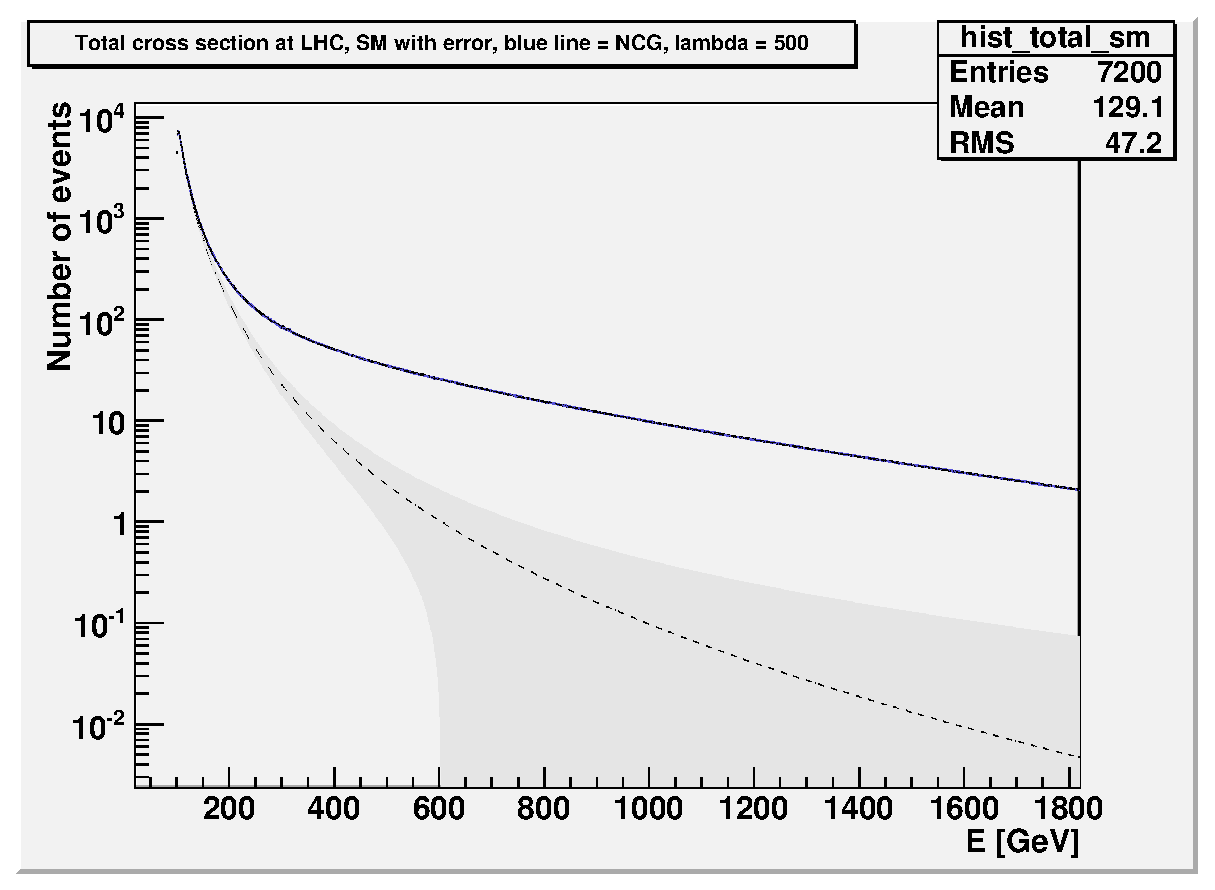
\includegraphics[scale=0.35]{./images/L500r139.eps}
	\end{minipage}
	%\hspace{0.5cm}
	\begin{minipage}[b]{0.475\linewidth}
    \centering
	  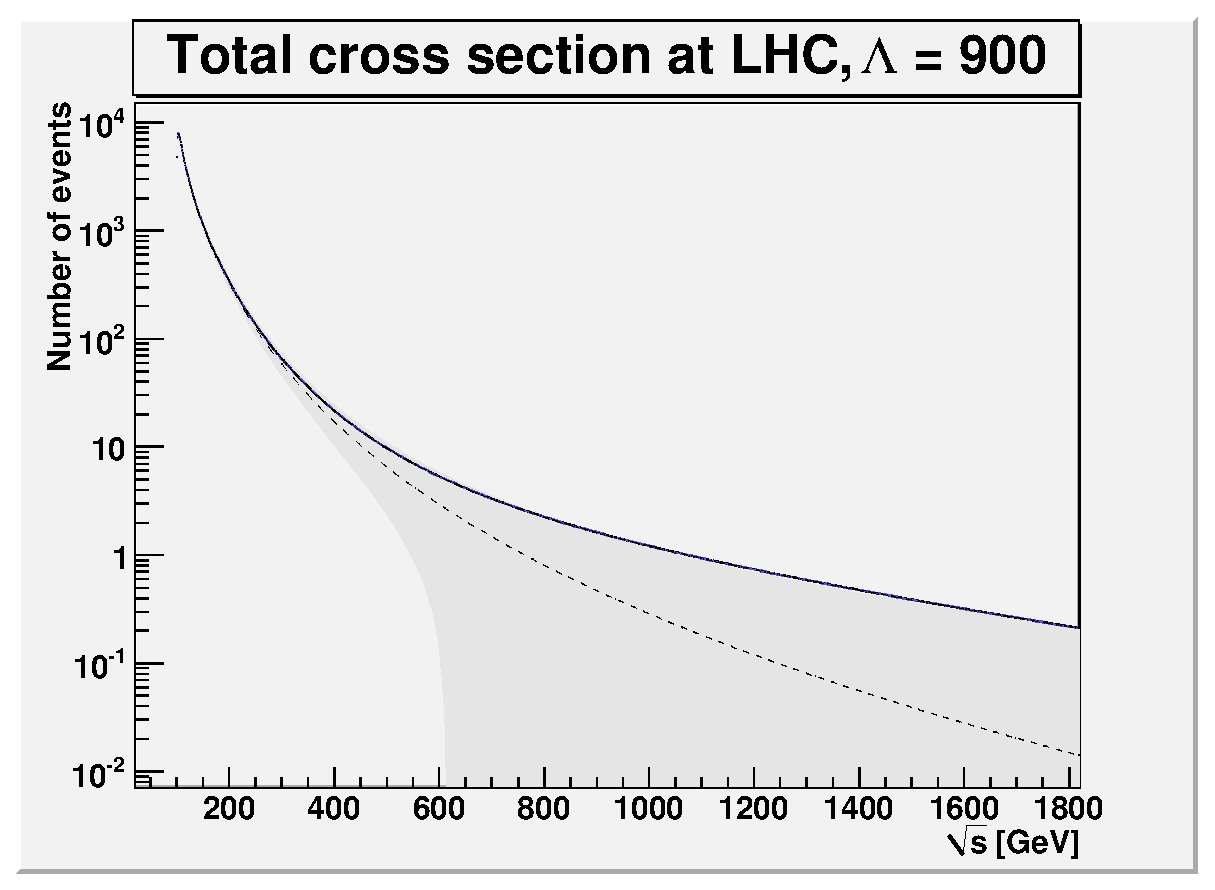
\includegraphics[scale=0.35]{./images/L900r139.eps}
	\end{minipage}
	\\ \vspace{0.5cm}
	\begin{minipage}[b]{0.475\linewidth}
    \centering
	  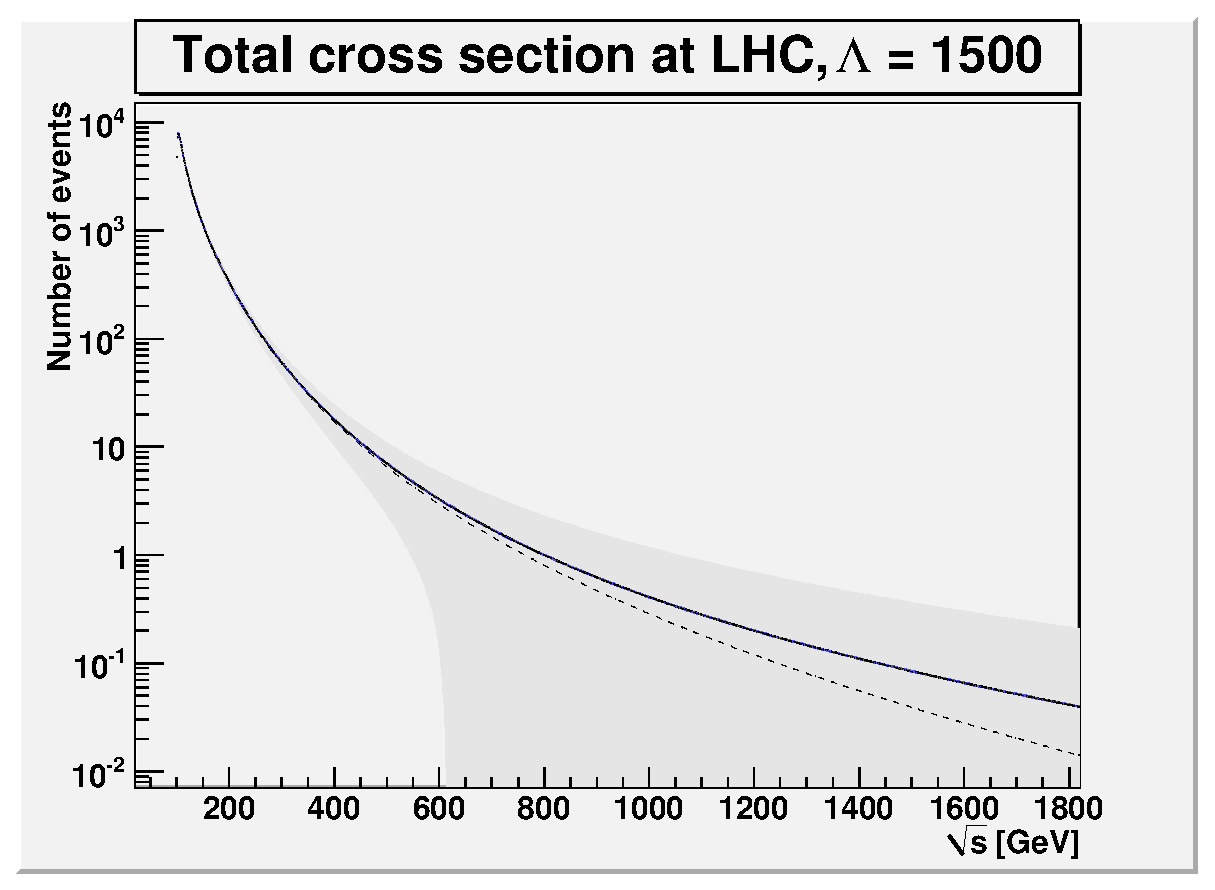
\includegraphics[scale=0.35]{./images/L1500r139.eps}
	\end{minipage}
	%\hspace{0.5cm}
	\begin{minipage}[b]{0.475\linewidth}
    \centering
	  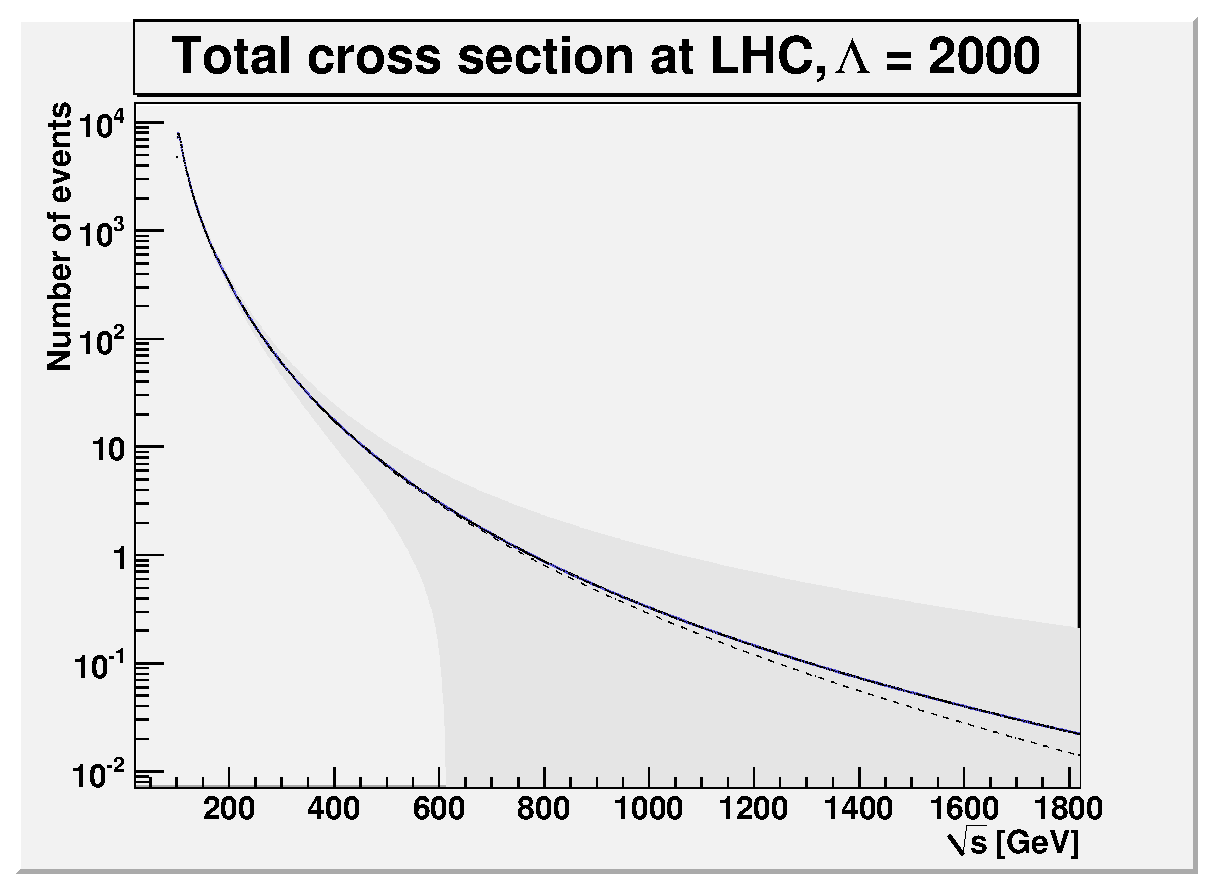
\includegraphics[scale=0.35]{./images/L2000r139.eps}
	\end{minipage}
		\caption{Predicted number of $pp \rightarrow Z/ \gamma \rightarrow \mu \bar \mu$ events at LHC running with a luminosity of $L=10 \textrm{ fb}^{-1}$ for one year. The grey line shows number of events as predicted by the SM with error $1.64\sigma = 1.64\sqrt{N}$, where $N$ is the number of events in the given bin. The blue line represent number of events as predicted by NCG for the given value of $\Lambda$. All interference terms and possible NCG contributions from $\gamma gg$ vertices have been ignored. Strictly speaking the histograms should have been cut off for $\sqrt{s} > \Lambda$, above which our approximation in the best case can be regarded as an extrapolation of a low energy effective theory.} \label{fig:lambdaplot}
\end{figure}
We have made histograms showing the expected number of muon-pair production events at LHC with integrated luminosity of $10 \textrm{ fb}^{-1}$ running for 1 year.\footnote{To get from cross section to $N$ we simply multiply the histograms by $10^4$ fb $\cdot$ pb$^{-1}$.} The distributions are made using leading order diagrams in CompHEP (Figures \ref{fig:feyn:parton_qq} and \ref{fig:feyn:parton_gg}) for the process $pp \rightarrow Z \rightarrow \mu \bar \mu$. All interference terms have been ignored. As have contributions from diagrams involving vertices $\gamma gg$. Four different plots are made for different values of $\Lambda$. The statistical error, $1.64\sqrt{N}$, where $N$ is the number of events in the given bin, is shown by the gray band for the ordinary SM data. Cross sections with contributions from NCG are shown as a blue line.

Note that we have made all plots up to an energy of $\sqrt{s} \sim 1800$ GeV, even though we made an approximation, in the zero-range interaction scheme, valid only for $\sqrt{s} \ll \Lambda$.\footnote{See the derivation in section \ref{sec:derivcrosssection}.} In the complete description we would expect a modification, perhaps even a resonance structure, of the NCG cross section in the region of $\sqrt{s} = \Lambda$. Our approximation ignores this behavior completely and instead we obtain an extrapolation of the low energy behavior for $\sqrt{s} \ll \Lambda$. This extrapolation can still be instructive to look at even for high energies where our approximation no longer holds.

Looking at the diagram for $\Lambda = 500$ we see that the effect of NCG should be clearly visible for energies above 200 GeV. Moving towards $\Lambda = 1000$ the NCG cross section approaches the 95\% CL on the SM data. At this scale, of 1000 GeV, NCG should still be visible as a systematic anomaly.\footnote{When calculating the $\chi^2$, we sum over the difference between observed and calculated values.} Approaching $\Lambda = 1500$ GeV our ability to observe NCG becomes questionable. In the case where we do not detect any contribution to the SM cross section.

We estimate, by looking at the plots, that the lower limit of $\Lambda$ should be be in area of 1000 to 1500 GeV.

The next step in the analysis would be to determine $\Lambda$ by a fit to the SM data and extract a corresponding limit. We have tried to do this in ROOT but ran into technical problems, which we were unable to resolve before the deadline.